\documentclass{sig-alternate}

% UTF8 support
\usepackage[utf8x]{inputenc}


\usepackage{hyperref}
\usepackage{epsf,graphicx}
\graphicspath{{figures/}}
\usepackage{subfigure}
%\usepackage[colorinlistoftodos]{todonotes}

\usepackage[usenames,dvipsnames]{xcolor}
\usepackage{tikz}
\usetikzlibrary{positioning, calc}


\newcommand{\eg}{{\textit{e.g.~}}}
\newcommand{\etal}{{\textit{et al.~}}}
\newcommand{\ie}{{\textit{i.e.~}}}

%
% --- Author Metadata here ---
\conferenceinfo{10th ACM/IEEE International Conference on Human-Robot Interaction}{2015 Portland, USA}
%\CopyrightYear{2007} % Allows default copyright year (20XX) to be over-ridden - IF NEED BE.
%\crdata{0-12345-67-8/90/01}  % Allows default copyright data (0-89791-88-6/97/05) to be over-ridden - IF NEED BE.
% --- End of Author Metadata ---

\title{\LARGE \bf
A Teachable Robotic Agent for Children Learning Handwriting, Capable of Simulated Handwriting Itself %make better
}

\numberofauthors{3} 
\author{
\alignauthor
Deanna Hood\\
Séverin Lemaignan\\
Pierre Dillenbourg\\
   \affaddr{Computer-Human Interaction in Learning and Instruction Laboratory (CHILI)}\\
   \affaddr{École Polytechnique Fédérale\\ de Lausanne (EPFL)}\\
   %\affaddr{CH-1015 Lausanne, Switzerland}\\
   \email{firstname.lastname@epfl.ch}
% \alignauthor
% Rafael Garcia\\
%    \affaddr{Computer Vision and Robotics Group (ViCOROB)}\\
%    \affaddr{University of Girona}\\
%    \affaddr{Girona, Spain}
}

%(DH) my EPFL email address won't work for much longer....


\begin{document}



\maketitle

%%%%%%%%%%%%%%%%%%%%%%%%%%%%%%%%%%%%%%%%%%%%%%%%%%%%%%%%%%%%%%%%%%%%%%%%%%%%%%%%
\begin{abstract}

%%% HRI 2015 -> double-blind review process

%Despite the social motivation for the use of a teachable agent for the
%engagement and support of children with handwriting difficulties, to date no
%such technology is known to have been developed. 

%(DH) abstract probably too long...
%(DH) do we have to be specific somewhere about what stage of handwriting we're targeting..?

This article presents the first known robotic partner which children can teach handwriting. It is
hypothesised that such a system could not just engage an unmotivated student,
but could also present the opportunity for children to experience the typical
benefits encountered during human-led handwriting interventions, such as motor
mimicry. Moreover, this system allows for exploring the potential for the
\emph{learning by teaching} paradigm to be employed in the interaction, so as to
stimulate meta-cognition, empathy and increased self-esteem in the child user. 

By leveraging simulated handwriting on a synchronised tablet display, a {\sc nao}
humanoid robot with limited fine motor capabilities has been configured as a
suitably embodied handwriting partner. Shape models derived from principal
component analysis of a dataset of letter trajectories have been generated, and allow
the robot to draw purposefully deformed letters. Learning how to write
characters well is then achieved by incorporating feedback from user
demonstrations, which allows the system to learn the optimal parameters for the
appropriate shape models. 

Preliminary in situ studies have been conducted with primary school classes to obtain
insight into children's use of the novel system. 
Children aged 6-8 were successfully able to engage with the robot and to improve its 
writing to a level which they were satisfied with. The validation of the interaction
represents a significant step towards an innovative use for robotics which addresses a
widespread and socially meaningful challenge in education. 

%, and provides context
%for robotics in education beyond the well-explored use of teaching coding and
%robotics-related subjects.

\end{abstract}


%%%%%%%%%%%%%%%%%%%%%%%%%%%%%%%%%%%%%%%%%%%%%%%%%%%%%%%%%%%%%%%%%%%%%%%%%%%%%%%%
\section{INTRODUCTION}

Handwriting difficulties in children at an early age often negatively affect
the academic performance of the students \cite{Christensen2005}, in addition to
their self-esteem being adversely affected \cite{Malloy1995}, causing them to
shy away from expressing what they know \cite{Medwell2008}.
%A conclusion drawn
%in \cite{Hoy2011} is that any handwriting intervention studies considered in the
%systematic review which involved fewer than two practice sessions per week and
%fewer than a total of 20 practice sessions, including homework, were found to
%demonstrate ineffective results. This highlights the necessity to engage
%students in an interaction that will be sustainable over the long-term. 
Successful interventions for children with handwriting difficulties involve the
student in many sessions where they are engaged in physically practising the
skill \cite{Hoy2011}. However, the link between handwriting difficulties and low
self-efficacy \cite{Engel-Yeger2009} results in children who are unmotivated to
participate in such sessions, potentially leading to a developmental arrest in
the acquisition of the skill. 

%Engel-Yeger, Nagauker-Yanuv and Rosenblum \cite{Engel-Yeger2009} have shown the
%link between handwriting difficulties and low self-efficacy, the belief in
%one's capabilities to complete a task. Bandura \cite{Bandura1990} maintains
%that self-efficacy constitutes the basis for the choice of whether or not to
%attempt a task. Indeed, third graders receiving intervention for their
%handwriting skills in \cite{Berninger1997} spoke of how they avoid writing
%because of how it is illegible to others. This mindset of believing that one is
%unable to write may lead to a developmental arrest in the acquisition of this
%skill, which may make intervention more difficult in the future. Consequently,
%it is of importance to engage students in activities in which their
%self-efficacy and self-motivation is restored.

The \emph{learning by teaching} paradigm, which engages the target student in
the act of teaching another, has been shown to produce motivational,
meta-cognitive, and educational benefits in a range of disciplines
\cite{Rohrbeck2003}. An application which is yet to be explored, however, is
that of handwriting intervention. One reason why this has not been investigated
to date may be that in order to engage a child in the learning by teaching
paradigm, there must be an appropriately unskilled peer for them to tutor. In
the context where the target child is the lowest performer in their class, this
may present a logistical constraint. In some cases, it may be appropriate for a
peer or teacher to simulate a na\"ive learner for the target child to teach,
however for an activity where one's skill level is visually evident -- as is the
case in handwriting -- this acting is likely to be eventually detected. As such,
there is motivation for the use of a teachable agent which can be configured for
a variety of skill levels, and for which children do not have preconceptions
about its handwriting ability.

Presented is the development of the first known teachable agent which is capable
of artificially making mistakes typical of children learning handwriting, and
correcting them with external feedback. Such a system therefore exhibits the potential
to engage children in the learning by teaching paradigm in the context of
handwriting. 

The teachable agent developed has the potential to be embedded as a simulated 
computer-based agent, however there are three main points which have motivated 
the use of a robot instead as the teachable agent in the presented work:

\begin{enumerate}
    \item the engagement and ``protégé effect'' elicited by teaching an embodied
        agent is anticipated to be stronger than that associated with a
        tablet-based application, which children are increasingly recognising as
        disposable technology,% * <deanna.m.hood@gmail.com> 2014-09-08T11:07:10.004Z:
%
% ... citation needed?
%

    \item observing a teachable agent respond to what it has been taught
        is a significant step in the learning by teaching
        paradigm \cite{Okita2006}, and therefore it may be significant for the agent to respond
        with a physical writing \emph{process}, rather than simply a product, and

    \item the potential for motor mimicry to yield significant improvements in
        handwriting interventions in which letter formations are demonstrated to participants \cite{Berninger1997} further supports the case
        for investigating the use of a humanoid robot capable of physically
        demonstrating handwriting trajectories to its child learning partner.
\end{enumerate}

Consequently, the learning agent developed has been embodied in a commercially
affordable {\sc nao} humanoid robot. Its writing capabilities have been implemented by
leveraging synchronisation with a tablet display to simulate fine motor skills
otherwise infeasible for the robot. 

Within this article, Section \ref{sec:learningAlgorithm} presents the novel work in the area of
artificial intelligence to develop a learning algorithm suitable for a teachable
agent in the context of handwriting. Section \ref{sec:robotWriting} details the
extension of this algorithm to an embodied robotic learning agent, including the
new approach for achieving simulated fine motor skills on commercially
affordable humanoid robots.  Section \ref{sec:experiment} explores the 
contributions made to the study of human-robot interaction, in discussing the
use of the first-of-its-kind system with primary school children and its potential as a tool for
addressing wider pedagogical research questions in education. Finally, Section \ref{sec:futureWork} addresses the challenges which are faced in extending this system to a level suitable for long-term studies, and Section \ref{sec:conclusions} concludes by reiterating the content and impact of the article's contributions.



%%%%%%%%%%%%%%%%%%%%%%%%%%%%%%%%%%%%%%%%%%%%%%%%%%%%%%%%%%%%%%%%%%%%%%%%%%%%%%%%
\section{A Learning Agent in the Context of Handwriting} \label{sec:learningAlgorithm}

For the development of a learning algorithm in the context of
handwriting, a parameterisation of letters and their deformities was sought such 
that different quality shapes can be generated, depending on the parameters input to
the letter models. This allows the system to be configured to improve its writing 
by modifying the parameters used to generate the letters, based on feedback from the 
reinforcement learning partner as addressed in Section \ref{sec:learningAlg}. 
%To this end, a method which can generate a model from real-world data
%has been employed in order to capture realistic variations in letters. 

\subsection{Shape Modelling of Letters} \label{sec:writingGeneration}

One approach for a shape model which can appropriately represent realistic
variations in shapes is statistical shape
modelling. Statistical shape modelling is an application of principle component
analysis (PCA), where a linear transform which de-correlates data vectors is
found \cite{Stegmann2002} and allows for dimensionality reduction. 

PCA has been performed on a set of letter paths captured from a digital pen,
using the UJI Pen Characters 2 dataset \cite{Llorens2008} with 120 instances of
each letter (2 repetitions from 60 adult users). While it may be appropriate in future work to
identify the location of salient features of the shapes which are robust to unanticipated user input,
the features are currently taken as $n$ uniformly spaced points along the shape
path. The
points are arranged into an observation vector presented in (\ref{eq:obsVec}),
where $x_i$ and $y_i$ represent the coordinates of each of the points along the
path. The observation shapes are normalised to have a unit maximum dimension 
and centre at the origin.

\begin{equation}\label{eq:obsVec}
{\bf x} = [x_1, x_2, \ldots, x_n, y_1, y_2, \ldots, y_n]^T
\end{equation}


The projection from the original $2n$-dimensional feature space $(n=70)$ to a reduced
$N$-dimensional space is found as in (\ref{eq:projection}), where ${\bf p}$
contains the coordinates in the $N$-dimensional space with ${\bf 0}$-origin,
calculated as in (\ref{eq:paramCalc}). The $2n\times N$ matrix ${\bf \Phi }$ is
an orthogonal matrix composed of the eigenvectors ${\bf v}_i$ corresponding to
the largest $N$ eigenvalues ($\lambda_i$) of the covariance matrix of the
observations, as shown in (\ref{eq:transformCalc}) \cite{Stegmann2002}. As such,
each shape may be approximated by the mean shape plus a sum of the top $N$
eigenvectors, weighted by the parameter vector ${\bf p}$. 

\begin{equation}\label{eq:projection}
{\bf \tilde{x}=\bar{x}+\Phi p}
\end{equation}
\begin{equation}\label{eq:paramCalc}
{\bf p} ={\bf \Phi}^T ({\bf {x}-\bar{x}})
\end{equation}
\begin{equation}\label{eq:transformCalc}
{\bf \Phi} = [{\bf v}_1, {\bf v}_2, \ldots, {\bf v}_N]^T
\end{equation}

If there is correlation between the points in the observations, there will be
eigenvalues of the covariance matrix which are close to zero. As such, removing
the associated eigenvectors from ${\bf \Phi}$ allows for dimensionality
reduction with minimal impact. 
%Indeed, the amount of variance in the dataset
%that is explained by each eigenvector ${\bf v}_i$ is $\sqrt{\lambda_i}$, and
%therefore the proportion of the variance explained by each dimension/eigenvector
%is as shown in (\ref{eq:proportionVar}).
%
%\begin{equation}\label{eq:proportionVar}
%\%var_i = \frac{\sqrt{\lambda_i}}{\sum_{i=1}^{N}\sqrt{\lambda_i}}\times 100\%
%\end{equation}

For the dataset presented in Figure \ref{fig:deviations_sPrint}, the
eigenvectors associated with the 3 largest eigenvalues explain 78.5\% of the
variance in the dataset, illustrating the capability of the statistical shape
modelling approach to produce compact parameterisation of shapes. 

%Clusters within paths of a particular letter have been identified using K-means
%clustering to group different styles of writing the letter (\emph{allographs}),
%such that the parameters in the resulting model are only representative of the
%specific allograph of the letter in the dataset. 
% * <deanna.m.hood@gmail.com> 2014-09-03T13:05:23.576Z:
%
% in the end this was pointless so maybe not worth mentioning
%
PCA has been performed on all of the paths of a particular allograph in the
dataset individually, to reduce the $2n$-dimensional space to one of a desired
number of dimensions. $N=10$ has been used for the work presented.

(\ref{eq:projection}) may also be used
to generate new shapes based on the parameters ${\bf p}$ which are used. ${\bf
p}={\bf 0}$ will yield the mean shape, and variations to each of the $N$ values
in ${\bf p}$ will cause a change in the shape represented by the corresponding
eigenvector (Figure \ref{fig:deviations_sPrint}). 

\begin{figure}[thpb]
\centering
\subfigure{
\raisebox{-0.5\height}{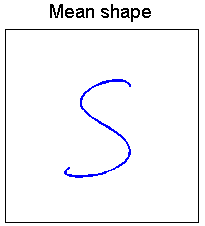
\includegraphics[width=0.05\textwidth]{figures/sPrint_mean.png}
}}
\subfigure{
\raisebox{-0.5\height}{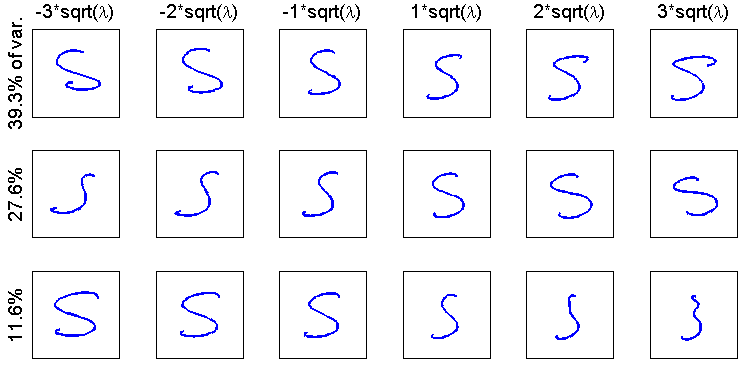
\includegraphics[width=0.35\textwidth]{figures/sPrint_top3.png}
}}
\caption[The mean shape and the effect of varying the first three parameters of
the shape model derived from PCA from the dataset of print `s'
shapes.]{\label{fig:deviations_sPrint}The mean shape (left) and the effect
    (right) of varying the first three parameters (each row) of a shape model.
     The extent to which each
parameter is varied is dependent on the eigenvalue $\lambda$ corresponding to
the parameter's eigenvector. The percentage of the total variance in the dataset
explained by each parameter is shown to the left of the corresponding row. }

\end{figure}

Interestingly, although the parameters are the result of an \emph{unsupervised}
statistical shape analysis, they still represent variations which could have
been intuitively identified by a manual parameterisation. For example, for the
model shown in Figure \ref{fig:deviations_sPrint}, the parameters may represent
the height of the top half of the letter compared to the bottom half, the width
of the overall shape, etc. The ability to create varied levels of deformations
which may be ascribed descriptive interpretations (not just numerical) is an
advantage of this method, given its context of use. If a teacher wishes to
create initial letters with a particular feature (a wide `s' or a `d' with a
large loop, for example), it is possible with this system. 


\subsection{Generating Poor Letters}

After determining the appropriate number of dimensions ($N$) for the shape
models, new letters can be generated by varying the parameter values in this
$N$-dimensional space in accordance with (\ref{eq:projection}). By choosing
parameter values which lie within the observed range in the dataset, it is
possible to produce letters which are more likely to be reasonable looking.
When the parameter values are outside of the range observed in the dataset, they
are less likely to represent shapes from the dataset of adult-written letters, 
and as a result are more likely to represent poor shapes.
Figure \ref{fig:sampleLetters} illustrates sample letters generated from the
models of `e' and `g' by selecting random values for the first 5 parameters 
from a distribution with
standard deviation of $3\sqrt\lambda_i$ rather than the $\sqrt\lambda_i$
standard deviation observed in the dataset.

\begin{figure}[thpb]
\centering
\subfigure{\raisebox{-0.5\height}{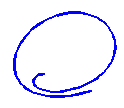
\includegraphics[height=0.04\textwidth]{figures/e1.png}}}
\subfigure{\raisebox{-0.5\height}{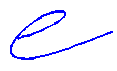
\includegraphics[height=0.025\textwidth]{figures/e4.png}}}
\subfigure{\raisebox{-0.5\height}{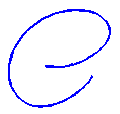
\includegraphics[height=0.04\textwidth]{figures/e3.png}}}
\subfigure{\raisebox{-0.5\height}{
\includegraphics[height=0.04\textwidth]{figures/e5.png}}}~~~~~
\subfigure{\raisebox{-0.5\height}{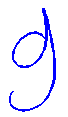
\includegraphics[height=0.06\textwidth]{figures/g1.png}}}
\subfigure{\raisebox{-0.5\height}{
\includegraphics[height=0.06\textwidth]{figures/g3.png}}}
\subfigure{\raisebox{-0.5\height}{
\includegraphics[height=0.06\textwidth]{figures/g4.png}}}
\subfigure{\raisebox{-0.5\height}{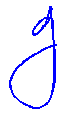
\includegraphics[height=0.06\textwidth]{figures/g5.png}}}
\caption[Sample letters generated from the PCA shape model on `e' and `g'
paths.]{\label{fig:sampleLetters}Sample letters generated from the PCA shape
model on `e' (left) and `g' paths (right), generated randomly from
parameters with $3\times$ the standard deviation observed in the dataset.}

\end{figure}

In \cite{Chandra2013}, it was found that children aged 4-6 years participating
in a handwriting peer tutoring pilot study most often made mistakes classified
as inappropriate \emph{internal proportions} or \emph{global deformations}. It
would be reasonable to consider the shapes in Figure \ref{fig:sampleLetters} in
the same general categories. Using a database of children's letters when
available may yield potential for parameterising other mistakes made by
children, such as merging strokes or decomposing a shape into multiple subparts
inappropriately. Nevertheless, sufficient capabilities for the shape model to
generate `poor' letters which are appropriate for simulating a na\"ive learner
in the context of handwriting have been demonstrated, using the shape model
generated from PCA on a dataset of only adults' writing.


\subsection{Responding to Feedback}\label{sec:learningAlg}

It was shown in Section \ref{sec:writingGeneration} how the statistical shape
model of a particular letter may convert a set of parameters into a generated
letter. Similarly, the model may also be used ``in reverse'' 
to convert a
letter into its parameters, given the model. The parameters of user-drawn
letters may therefore be used in order to incorporate the capabilities for the
learning algorithm to adapt to the user's feedback via demonstration.

The statistical shape model may be used to determine the parameters of a
demonstration shape by projecting the features of the observed shape into the
lower-dimensional space determined by the model. Mathematically, given a
demonstration ${\bf x}_{demo}$, the associated parameters may be determined as in
(\ref{eq:param}).

\begin{equation}\label{eq:param}
{\bf p}_{demo} ={\bf \Phi}^T ({\bf{x}_{demo}}-\bf{\bar{x}})
\end{equation}

The parameters which are determined for a shape in (\ref{eq:param}) will not
reconstruct the shape exactly if $N<2n$, but rather will reconstruct the closest
point in the $N$-dimensional space which the eigenvectors span.

For the statistical shape model employed by the system, the method for
responding to user demonstrations is to move the learning algorithm's parameters
towards those of the demonstration. In the results presented in this work, the
linear update equation shown in (\ref{eq:update}) has been used, where ${\bf p}$ is the
learned parameter vector at time step $k$, and $\alpha$ is the learning rate,
between 0 and 1.  

\begin{equation}\label{eq:update}
{\bf p}^{(k+1)} = {\bf p}^{(k)} + ({\bf p}_{demo}-{\bf
p}^{(k)})\times\alpha
\end{equation}

Figure \ref{fig:demonstrationShapes2} illustrates the response of the system to
demonstrations from a child for the letter `s' using a learning rate of
$\alpha=1/2$.  Note that even poorly-written demonstrations allow the system to improve.

\begin{figure}[thpb]
    \centering
    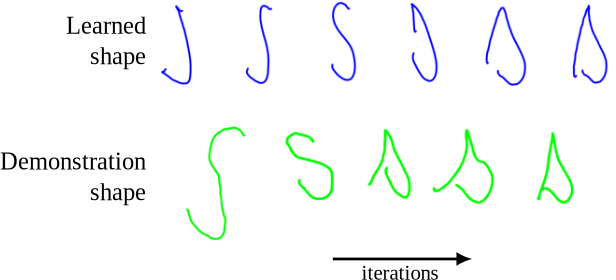
\includegraphics[width=0.45\textwidth]{figures/learningSdemo}
    \caption{\label{fig:demonstrationShapes2}Example of the learning algorithm
    responding (top) to user demonstration of shapes (bottom) for the letter `s' (demonstrations received from two 7-8 year-old children taking turns).}
\end{figure}

It is possible that parameters ${\bf p}^{(k)}$ and ${\bf p}_{demo}$, which
individually yield acceptable shapes, produce parameters ${\bf p}^{(k+1)}$
which yield an unacceptable shape. This is especially true if the demonstration
shape is of a different style to that learnt at time $k$, as there are no
restrictions imposed on parameter values. However, the proposed method for adapting to
the demonstration shapes has the advantage of being able to recover from such a situation: with further
demonstrations of the same letter, the system would eventually approach the
demonstration shape (see Figure \ref{fig:eDemo}. As a result, the event of poor-looking 
intermediate letters
would not limit the interaction later proposed in Section \ref{sec:experiment}
in a technical sense, but it may influence the user's \emph{perception} of the learning
agent. It remains to be seen if it is necessary to avoid such an event
mathematically.

\begin{figure}[thpb]
    \centering
    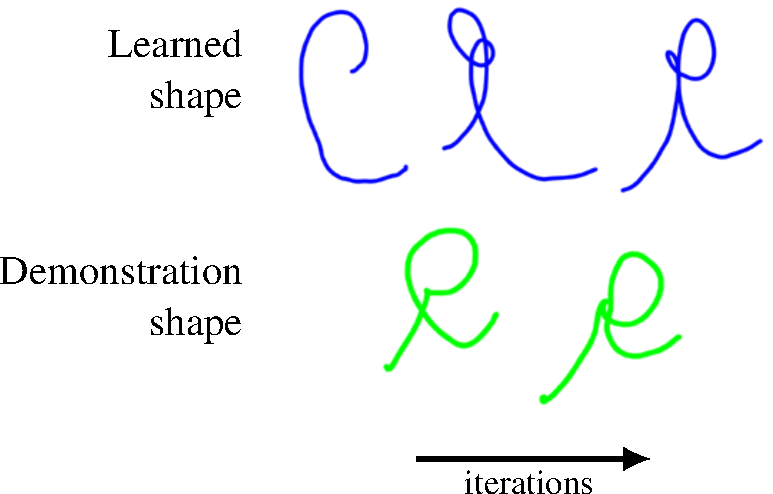
\includegraphics[width=0.3\textwidth]{figures/learningEdemo}
    \caption{\label{fig:eDemo}Example of the learning algorithm
    responding (top) to user demonstration of shapes (bottom) for the letter `e', passing through a parameter state which yields a poor letter (demonstrations received from a 7-8 year-old child).}
\end{figure}



%%%%%%%%%%%%%%%%%%%%%%%%%%%%%%%%%%%%%%%%%%%%%%%%%%%%%%%%%%%%%%%%%%%%%%%%%%%%%%%%
\section{An Embodied Handwriting Learning Agent with the NAO Humanoid Robot}
\label{sec:robotWriting}

In order to develop a teachable agent that is appropriate for engaging a child
through the learning by teaching paradigm, 
%- that is, that it is an embodied agent, capable of eliciting motor mimicry,
%and capable of causing its teacher to reflect on the process that has been used
%to respond to handwriting feedback -
capabilities for the robot to engage in handwriting and interactive turn-taking have been established.

The {\sc nao} V4 humanoid robot, which has been developed by Aldebaran Robotics and 
purposely designed to look approachable \cite{Gouaillier2008}, has been used for
this work. It is a commercially affordable biped robot, 58cm tall, with 25
degrees of freedom, two cameras, speech capabilities and the ability to
autonomously execute a range of tasks.

%Because of the challenges in getting the {\sc nao} to write trajectories smoothly
%because of its inherent ability to only reach discrete points in space, 
Precise control over what the robot is writing is necessary in the
proposed application of a learning agent in this context. Because
of the limited fine motor skills possible with such an affordable robot, in
addition to the absence of force feedback and other technical necessities, the
{\sc nao} has been configured to use simulated handwriting with a synchronised tablet
to achieve this level of control. The necessary components of implementing the
proposed teachable robotic agent are, therefore:

\begin{enumerate}
    \item developing capabilities for the robot to trace handwriting ``in the air'', 

    \item synchronising the robot's movements with the display of the writing on a
        tablet so that it appears that the robot is causing the handwriting to
        display because of its actions, and

    \item integrating the writing behaviour with the handwriting learning
        algorithm presented in Section \ref{sec:learningAlgorithm} to create a
        \emph{learning by teaching} interaction with the agent. 
\end{enumerate}

These steps are presented in the sections which follow.

\subsection{Robot Trajectory Following}

Using simulated handwriting provides an opportunity for the robot's writing to
appear smoother than would be achievable with a writing instrument. However, the
robot's motions must still sufficiently match the displayed trajectory in order
capture the engagement of the child participant in the action. Aldebaran's NaoQi API
has been used for the inverse kinematics of the trajectory following. The Robot
Operating System (ROS)\footnote{The ROS stack for {\sc nao} is available at:
\url{http://wiki.ros.org/nao_robot}.} has been used for integration of the {\sc nao}
with external reference frames, such as the tablet's location, using the $tf$ transformation library \cite{Foote2013}.

When using simulated handwriting, it is no longer necessary that the robot
engages in the typical style of handwriting, with a writing instrument at a desk.
By instead having the robot point at a vertical writing surface to cause the
trajectory to appear (as in Figure \ref{fig:naoWriting}), several advantages are
presented:

\begin{itemize}

    \item The working space of the robot increases, both in the technical sense
        and the interaction sense: someone can, in theory, show the tablet to
        the robot from across the room and have it still respond, without
        needing the tablet to be within arm's reach.

    \item Concerns about whether or not the child would start mimicking the
        robot's incorrect writing form (\eg pen grip) are mitigated. 

    \item Perhaps most significantly, the accuracy of the matching of the
        robot's motion with the trajectory displayed on the tablet is not as
        critical, because the finger is not expected to touch the tablet exactly
        at the trajectory point, in contrast to a pen tip.
        % This means that orientation degrees of freedom can be freed without significant adverse effects.

\end{itemize}

\begin{figure}[thpb]
     \begin{center}
        %\subfigure{
        %    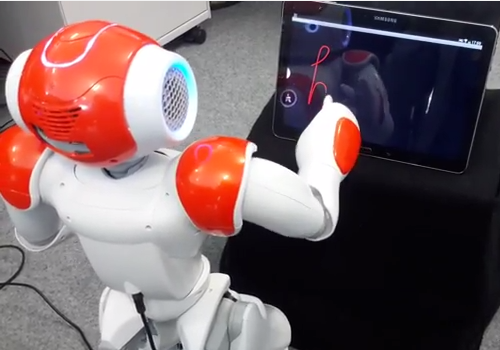
\includegraphics[width=0.4\textwidth]{figures/naoWriting1.png}
        %}%
        \subfigure{
            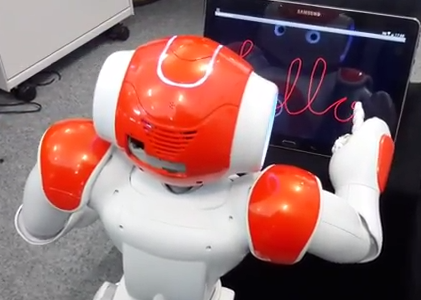
\includegraphics[width=0.6\linewidth]{figures/naoWriting2.png}
        }%
%
    \end{center}
    \caption{A demonstration of the robot simulating the writing of a word with
    its finger. The motion of the robot is synchronised with the display of the
    tablet, communicating over ROS.\protect\footnotemark}%

   \label{fig:naoWriting}
\end{figure}
\footnotetext{See \url{https://www.youtube.com/watch?v=2qWFSJRxCU0} for a video of the synchronised 
writing demonstration. }

Therefore, the system presented utilises the context where the robot is
simulating handwriting by pointing at the tablet\footnote{Teachers interviewed
for their feedback on the system advised that children are asked to draw letters
in the air in a similar manner as part of their handwriting education. The behaviour 
is hence not unfamiliar to children.}. As
interacting with a tablet with one's finger is not uncommon, this may aid the
acceptance of the writing style by users. 

Because
motion planning is performed with respect to the hand of the robot, rather than
its fingertip, one or two of the orientation degrees of freedom of the hand
are fixed to keep the finger approximately perpendicular to the writing surface,
depending on the desired accuracy. The remaining free orientation(s), coupled
with the whole-body motion control available, allow for a sufficient working
space for writing on the entire tablet.

\subsection{Synchronisation with the Tablet Trajectory Display}\label{sec:tabletSynch}

After getting the robot to trace writing trajectories, the next step towards
simulated handwriting is getting the trajectories of the robot's `writing' to
display on an Android tablet. 

ROS has been used for the communication between the devices used in the system,
including the Android tablet\footnote{For more information about ROS on Android
devices see \url{http://wiki.ros.org/android}}. As a result, aspects of the
networking between the tablet and the robot, such as the overheads associated
with connections, ports, message formats, etc. have been simplified. 

An Android application has been developed to receive the trajectory message over
a ROS topic and display the trajectory as an
animation. Synchronisation between the tablet and the robot has been achieved by:

\begin{itemize}

    \item sending a requested start time accompanying the trajectory, which is
        sufficiently in the future, to account for varying transmission delays
        to the nodes on different devices,

    \item synchronising all clocks with NTP servers such that the ROS time used
        for responding to the requested start time is the same at all nodes,

    \item reducing the number of points along the trajectory passed to the
        robot's motion planner to improve timing accuracy, and

    \item not running computationally expensive tasks on the robot (such as
        camera publishing) while it is writing as this interferes with the
        requested timings between points. 

\end{itemize}

To instruct the robot where to write, the robot has been configured to detect a
particular fiducial marker, a \emph{chilitag}\footnote{See
\url{https://github.com/chili-epfl/ros_markers} for more information on the
fiducial markers used.}, with the camera located in its head, and to use that to
determine the relative position of the writing surface (Figure
\ref{fig:tabletDetection}). When used in an interaction involving a participant, this
allows a user to move the tablet as required for the interaction. As broadcasting
the robot's camera has been identified as a computationally expensive task which
can disrupt the robot's timing of synchronised writing, it is only done when the
robot is not writing, and the tablet is assumed to be stationary during the
writing process.

\begin{figure}[htpb]
    \centering
    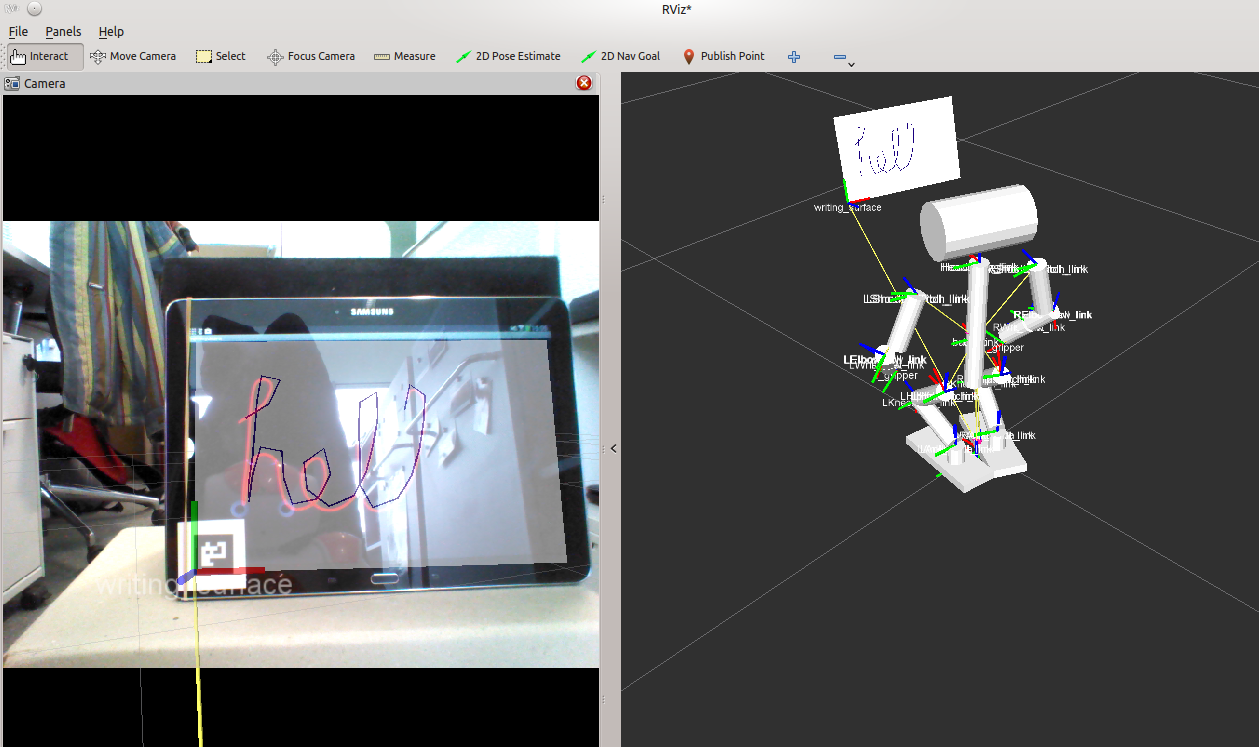
\includegraphics[width=0.35\textwidth]{figures/chilitagDetection_cameraOverlay.png}
    \caption{\label{fig:tabletDetection}Detection of the tablet using a fiducial
    marker to represent the origin of the writing surface frame, visualised in RViz. The robot's
    camera image is on the left, with the text trajectory overlay visible.}

\end{figure}


\subsection{Integration into a Robotic Agent}

The fusion of the embodied handwriting agent developed with the handwriting
learning algorithm presented in Section \ref{sec:learningAlgorithm} involves the
integration of three components: the robot, the tablet, and a central controller
(Figure~\ref{fig:archi}).  The robot and Android tablet application present the
writing process/result to the user, as in Section \ref{sec:tabletSynch}.
The tablet application has been extended to act as the primary medium for
capturing participant input, and publishes the user's demonstrations when they are
satisfied with their writing. The user demonstrations are received by the
interaction controller running on a desktop computer. It is responsible for
getting the {\sc nao} to prompt and respond appropriately to feedback received using
a finite state machine to manage the interaction stage and various system
inputs.  In the context of learning handwriting, an additional input to the system is a word 
from which the letters are to be learned, as detected by a fiducial marker on a word card.
The controller manages the learning algorithm by inferring the letter which
user demonstrations are intended for based on their position on the tablet, and
publishes the shapes to be written which are generated by the learning algorithm
in response to the feedback.  

The source code for the teachable robotic handwriting partner has been made 
available at \url{https://github.com/chili-epfl/cowriter_letter_learning}.


%Feedback from the user is passed to the controller with the location on the
%tablet that it occurred at, and the task of interpreting the shape which the
%feedback was intended for is left to the controller as it is aware of the
%location of published shapes. The appropriate response in terms of the learning
%algorithm is then taken for the respective shape. 


\begin{figure}[ht]
\centering

\resizebox{0.9\linewidth}{!}{%

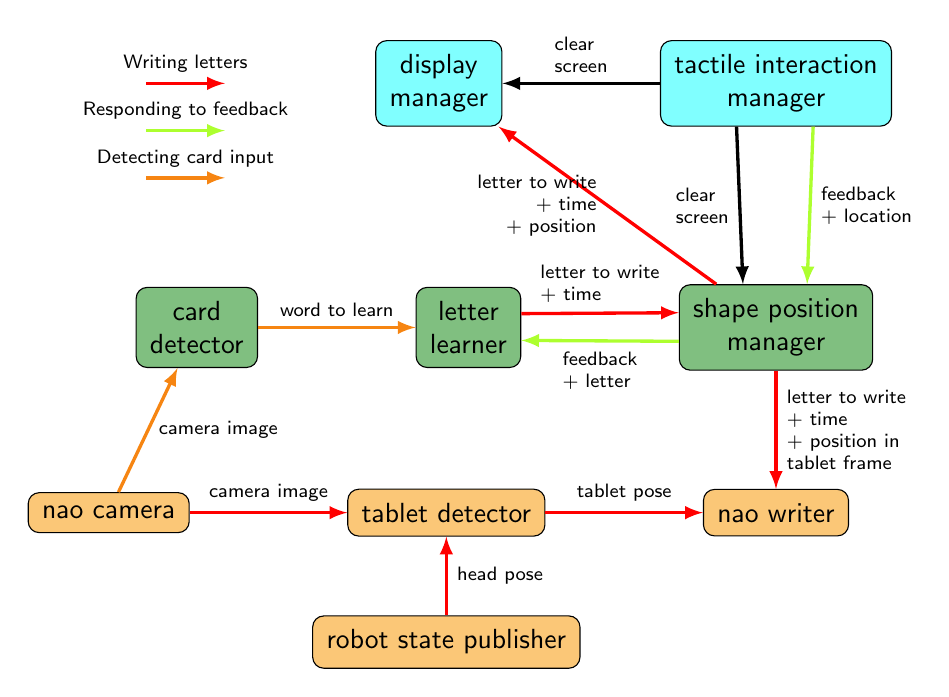
\begin{tikzpicture}[
    >=latex,
    node distance=2cm,
    every edge/.style={draw, very thick},
    redarrow/.style={fill=Red, draw=Red},
    greenarrow/.style={fill=GreenYellow, draw=GreenYellow},
    yellowarrow/.style={fill=BurntOrange, draw=BurntOrange},
    cmpt/.style={draw, align=center, rounded corners, inner sep=5pt, font=\sf, fill=black!20},
    label/.style={midway, align=left, font=\scriptsize\sf, fill=white, above,opacity=0,text opacity=1}]

    \node at (0,0)[cmpt, fill=Cyan!50] (tactile) {tactile interaction \\ manager};
    \node[cmpt, fill=Cyan!50, left=of tactile] (display) {display \\ manager};
  
    \node [cmpt, fill=Green!50, below=of tactile] (shape) {shape position \\ manager};
    \node [cmpt, fill=Green!50, left=of shape] (learner) {letter \\ learner};
    \node [cmpt, fill=Green!50, left=of learner] (card) {card \\ detector};

    \node [cmpt, fill=YellowOrange!50, below=1.5cm of shape] (writer) {nao writer};
    \node [cmpt, fill=YellowOrange!50, left=of writer] (tablet) {tablet detector};
    \node [cmpt, fill=YellowOrange!50, left=of tablet] (camera) {nao camera};
    \node [cmpt, fill=YellowOrange!50, below=1cm of tablet] (pose) {robot state publisher};

    %%% Relations between components
    \path (tactile) edge [->] node[label] {clear \\ screen} (display);

    \path ($(shape.north west)!0.33!(shape.north east)$) edge [<-] node[label,left] {clear \\ screen} ($(tactile.south west)!0.33!(tactile.south east)$);
    \path ($(shape.north west)!0.66!(shape.north east)$) edge [<-, greenarrow] node[label,right] {feedback \\ + location} ($(tactile.south west)!0.66!(tactile.south east)$);

    \path (shape) edge [->, redarrow] node[label, left, align=right] {letter to write \\ + time \\ + position} (display);
    \path (shape) edge [->,redarrow] node[label, right] {letter to write \\ + time \\ + position in\\tablet frame} (writer);

    \path ($(shape.north west)!0.66!(shape.south west)$) edge [->, greenarrow] node[label,below] {feedback \\ + letter} ($(learner.north east)!0.66!(learner.south east)$);
    \path ($(shape.north west)!0.33!(shape.south west)$) edge [<-, redarrow] node[label] {letter to write \\ + time} ($(learner.north east)!0.33!(learner.south east)$);

    \path (card) edge [->, yellowarrow] node[label] {word to learn} (learner);
    \path (camera) edge [->, yellowarrow] node[label, right] {camera image} (card);
    \path (camera) edge [->, redarrow] node[label] {camera image} (tablet);
    \path (tablet) edge [->, redarrow] node[label] {tablet pose} (writer);
    \path (pose) edge [->, redarrow] node[label, right] {head pose} (tablet);

    \path (-8, 0) edge [->, redarrow] node[label] {Writing letters} (-7, 0);
    \path (-8, -0.6) edge [->, greenarrow] node[label] {Responding to feedback} (-7, -0.6);
    \path (-8, -1.2) edge [->, yellowarrow] node[label] {Detecting card input} (-7, -1.2);
    
\end{tikzpicture}
}

\caption{Overview of the system. Components in the top row run on the tablet, 
those in the middle row on the central controller, and those in the bottom row 
on the robot.}

    \label{fig:archi}
\end{figure}



%%%%%%%%%%%%%%%%%%%%%%%%%%%%%%%%%%%%%%%%%%%%%%%%%%%%%%%%%%%%%%%%%%%%%%%%%%%%%%%%

%%%%%%%%%%%%%%%%%%%%%%%%%%%%%%%%%%%%%%%%%%%%%%%%%%%%%%%%%%%%%%%%%%%%%%%%%%%%%%%%

\section{A Tool for Social and Pedagogical Investigations} \label{sec:experiment}
\label{sec4}

In addition to constituting a technically novel system, the presented teachable
robotic agent represents a tool which may be used for investigating social and
pedagogical research questions. For example, one such question is what impact the addition of
such a teachable robotic agent would have on the outcomes of a typical
handwriting intervention. 

\subsection{Interaction Context}

The interaction context which has been developed as a framework for addressing
relevant research questions is one where participants are asked to improve the robot's
handwriting by correcting its letters. Figure~\ref{fig:pilotInteraction}
illustrates an example interaction sequence between the participant and the
robot which consists of the following stages:

\begin{enumerate}

    \item The participant shows the robot one of seven different 3-letter words
        to write, which, combined, consist of 7 different letters (`c', `e',
        `n', `o', `s', `u', `w'). Fiducial markers which are printed on the word
        cards allow them to be detected with the robot's camera. 

    \item The robot responds to the word request verbally and writes the
        letters by pointing at the tablet and imitating writing the letters. The
        tablet, placed in front of the robot with a vertical, landscape orientation,
        displays the letters in synchronisation with the robot's movements. 

    \item The robot asks for feedback from the participant and they demonstrate
        how to write the letter which they feel needs to be corrected. The
        demonstration is performed by drawing on the tablet with a stylus. The
        tablet may be moved into the most appropriate position for the child to
        write on it. Only one letter may be demonstrated at a time and the
        position of the participant's demonstration on the tablet encodes the
        letter that it is a demonstration for. The participant can remove and
        repeat their letter if they are unhappy with it.
        %, or if it is in the wrong position as determined by the researcher
        %conducting the interaction
        When the participant is satisfied with the demonstration, a button on
        the tablet which signals that it is the robot's turn is pressed and the
        demonstration is sent to the controller.

    \item The controller produces an adapted letter for the robot to write in
        response to the participant's feedback, and the interaction iterates,
        with participants taking turns to interact with the robot if necessary.
        When the participant(s) is/are satisfied with the robot's performance on 
	all letters,
        they may use the ``test'' card and an additional word for which they will
        verbally evaluate the robot's performance. 

\end{enumerate}

%To allow the system to take input from the user on which words to draw,
%fiducial markers were placed on cards which were detectable by a
%previously-developed ROS node processing a camera stream. A node which
%processed the fiducial markers detected was then created to convert the card
%detected into an appropriate message for the controller. 
	
\begin{figure}[thpb!]
     \begin{center}
%
        \subfigure[The user shows a card to the robot with a word to write.]{%
            \label{fig:first}
            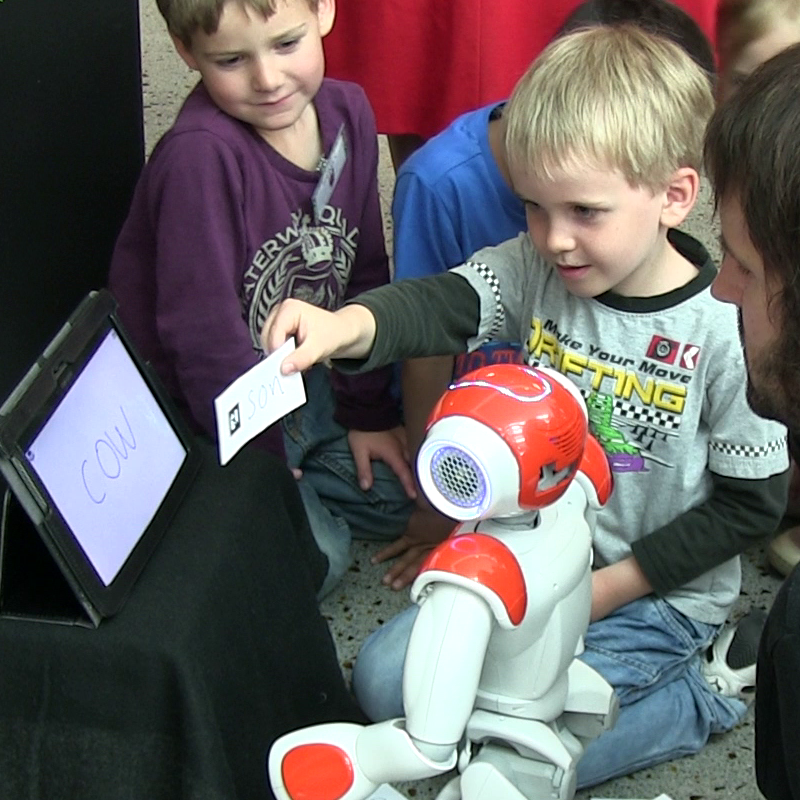
\includegraphics[width=0.2\textwidth]{figures/1card.png}
        }~
        \subfigure[The robot writes the word seen on the card and asks for feedback.]{%
           \label{fig:second}
           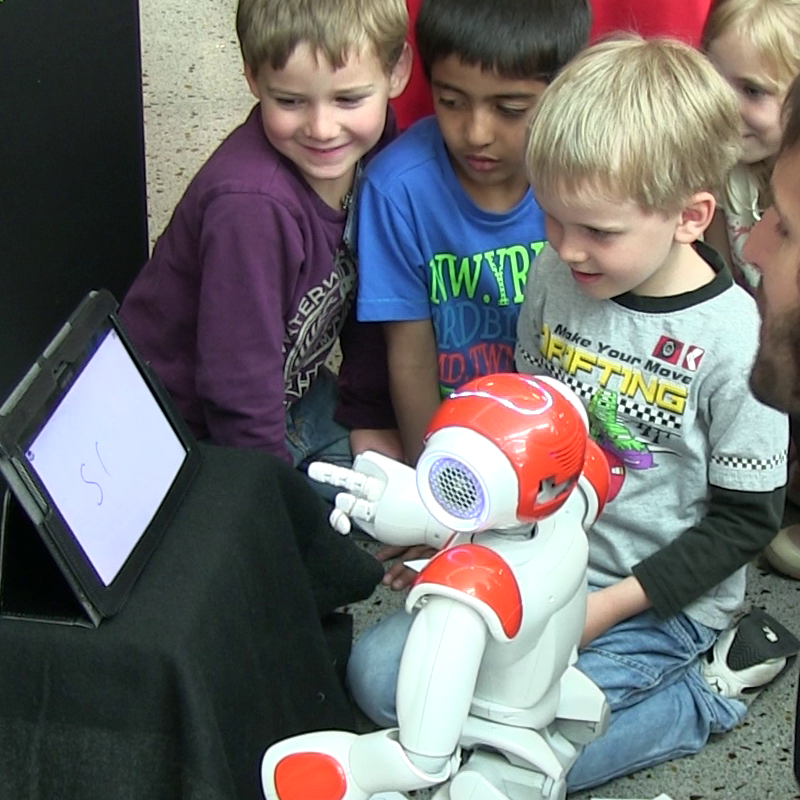
\includegraphics[width=0.2\textwidth]{figures/2word.png}
        }\\ %  ------- End of the first row ----------------------%
        \subfigure[The user provides feedback on the letters written via demonstration.]{%
            \label{fig:third}
            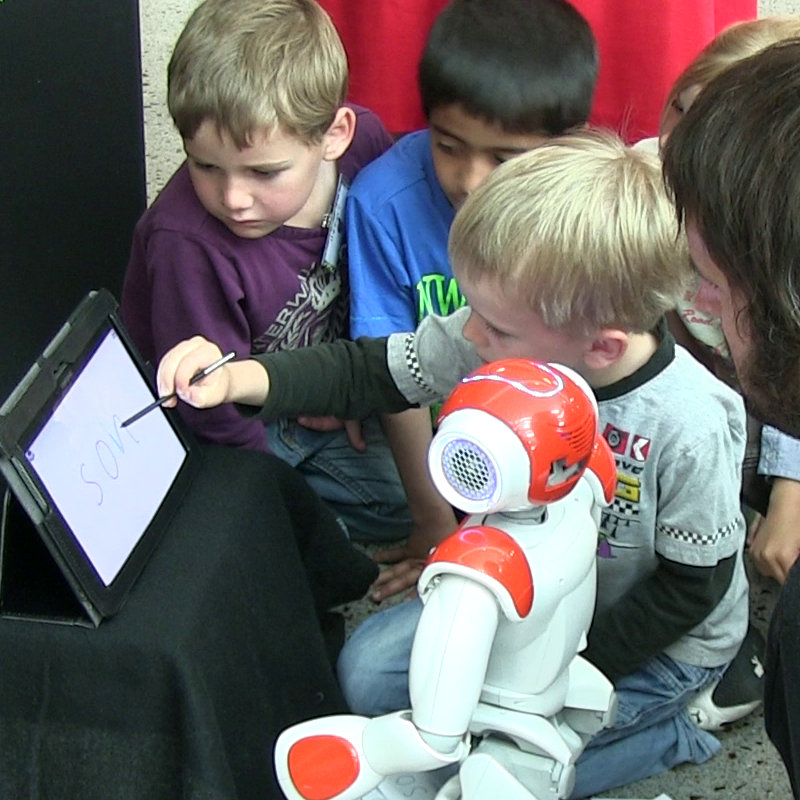
\includegraphics[width=0.2\textwidth]{figures/4correct.png}
        }~
        \subfigure[The robot responds to the feedback, until the user is satisfied.]{%
            \label{fig:fourth}
            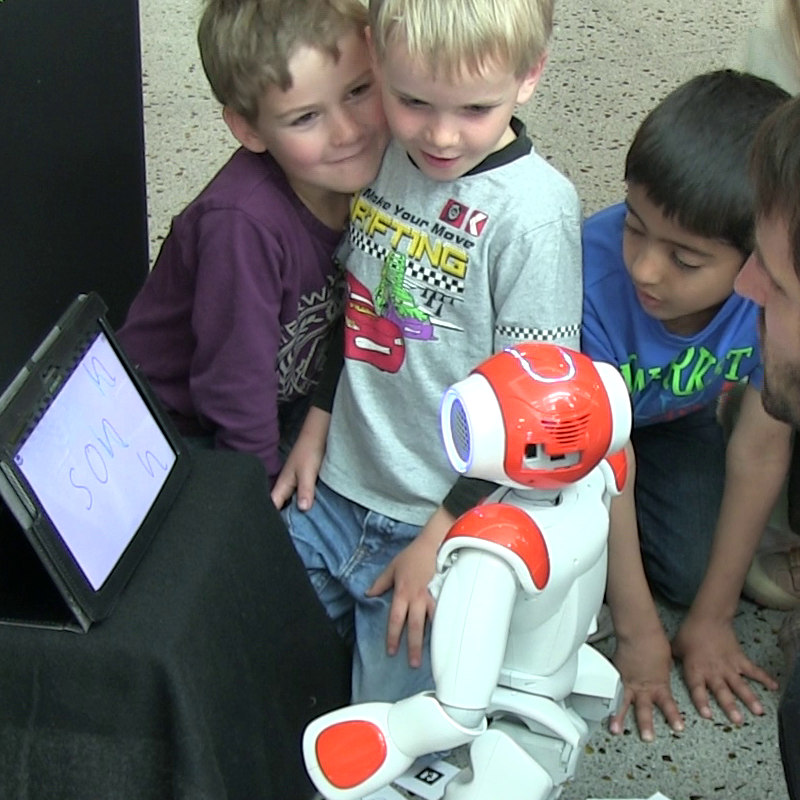
\includegraphics[width=0.2\textwidth]{figures/5iterateAsk.png}
        }%
%
    \end{center}
    \caption{%
        A user engaging with the robot in the \emph{learning by teaching}
    interaction, using demonstrations as feedback.}%

   \label{fig:pilotInteraction}
\end{figure}

\subsection{Outcomes of Preliminary Studies}

Preliminary studies at two schools in the Geneva area, involving more than 50 children, 
have been conducted to evaluate the feasibility and technical soundness of the 
interaction system proposed. 

A pilot study at the first school consisted of four groups of
approximately 8 english-speaking children, aged 6-7 years. The children
interacted with the system for a total of 65 minutes, with the robot writing 96
letters, of which 49 were in response to demonstrations from the children. 

As a result of the pilot study, two key observations were acted on. The first
was that children appeared to have a difficult time providing demonstrations to
the robot in the same place as previously-written letters. At the time, the
system required the children to write on top of a letter of the same type as the
one which they were demonstrating, and the children seemed to find this
counter-intuitive and would occasionally just trace the robot's letter as it
appeared. As such, the technical components of the system were extended to allow
the children the opportunity to write around previously-written letters instead
of on top. 

The second key point which came from the pilot study was that children were
observed giving advice to the child designated as the letter demonstrator,
potentially giving rise to the higher level paradigm of learning by
\emph{teaching to teach}. As a consequence of this observation, the study which
followed at the second school was designed to further observe the effect of the
number of children interacting with the robot.
%in order to investigate the potential of the system to not only be used to set
%the context of children tutoring the robot, but also children interacting as
%peer tutors with each other.

The study at the second school involved 21 french-speaking students aged 7-8 years: 7 children
interacted with the robot individually and 7 sessions included the remaining
14 students interacting with the robot in pairs. The duration of the sessions
was between 8 and 15 minutes, with an average of 11.4 minutes (SD = 2.3). 
Initial parameters were drawn from a range purposely chosen to generate shapes 
for letters 'e' and 's' which would elicit correction. For the other letters, 
parameters were fixed, generating shapes which some groups chose to correct 
(e.g. 13/14 for 'n' and 2/14 for 'c').

The following conclusions were successfully drawn about the system as a result
of the study at the second school.


    \textbf{The simulated robotic writing was believed by the children in all
    cases.} There were, at times, 
    % * <deanna.m.hood@gmail.com> 2014-09-05T11:59:03.640Z:
    %
    % how many
    %
    questions about the robot's writing method at the beginning of the interaction,
    but when advised that the robot ``tells the tablet what it wants to write,''
    this was accepted by the children. To allow the children an opportunity to
    express doubt in the robot's ability to write without explicitly asking them if
    the robot was pretending, the children were asked if they believed that the
    robot would be able to write its name, \emph{{\sc nao}} which had not previously been
    demonstrated. It was reasoned that this would prompt the children to question
    the point of the robot actually \emph{writing} if they had any suspicion that
    the robot was pretending, but this was never the case. In the event where the
    robot's writing was not correctly synchronised with the tablet, this did not affect the
    response of the child. If older children participate in the interaction study --
    which may be likely as children with lasting handwriting difficulties are included
    as participants -- it may become more important to invest time into the
    believability of the robot's writing scheme. However, for 6-8 year olds the
    proposed setup has been proven viable.

    \textbf{The children were engaged in teaching the robot.} % * <deanna.m.hood@gmail.com> 2014-09-05T09:54:48.069Z:
    %
    % maybe this is too strong as a 'conclusion' and should just be an observation. plus what does this even mean.. the child walking around the room was 'engaged' too...?
    %
    An average of 10.9 demonstration letters (SD = 4.4) were
    provided to the robot for each session during the interaction.
    In 9 out of the 14 sessions (64\%), the robot received demonstration letters
    \emph{after} reaching the test stage of the interaction. The participants'
    teaching after the test word had been written and evaluated -- the only
    purposefully imposed external motivation -- may suggest that by that time
    the participants had become intrinsically motivated to engage in the
    interaction.% * <deanna.m.hood@gmail.com> 2014-09-05T10:30:45.293Z:
    %
    % I guess it could have also come from us sitting there watching them
    %

    \textbf{All children believed that the robot was learning and that
        they were the ones teaching it.} This was concluded from the responses
        when the children were asked directly. This is in contrast to a prior
        feasibility study for a version of the interaction which only allowed
        for touch-based feedback, not user demonstrations, in which three of the
        seven adult participants did not feel that it was their input which
        helped the robot improve.
        % * <deanna.m.hood@gmail.com> 2014-09-05T09:46:49.117Z:
    %
    % probably can't just casually mention this study without going into more detail...
    %

    %, and also their reaction to the ``test word'' written by the robot at the end of the interaction. In X\% of cases, the child concluded that the robot had `passed' the test, or congratulated it in some way.


    \textbf{The system has been validated as a technically sound
        autonomous interaction.} The interaction setup including the teachable
        robotic agent withstood the interaction for a total of 160 minutes. During this
        time the robot wrote 335 letters, 152 of which in response to
        demonstrations received from the 21 children and the remaining while writing 
        new words. During this time, technical 
	intervention was only required for the three instances that the robot fell 
	later in the day. Otherwise, the technical components of the system operated 
	autonomously and as expected over the sessions.
        %, with only verbal interaction for prompting being required from an observing researcher.




%%%%%%%%%%%%%%%%%%%%%%%%%%%%%%%%%%%%%%%%%%%%%%%%%%%%%%%%%%%%%%%%%%%%%%%%%%%%%%%%
\section{Towards Long-term Interventions}\label{sec:futureWork}
%why is this title going into the margins....

A conclusion drawn in~\cite{Hoy2011} is that any 
handwriting intervention studies considered in the systematic review which involved 
fewer than two practice sessions per week and fewer than a total of 20 practice 
sessions, including homework, were not found to demonstrate effective results. This 
highlights the necessity to engage students in an interaction which will be sustainable
 over the long-term in order to answer 
research questions which involve the measurement of learning gains. 
Several challenges are raised in developing such long-term capabilities for the system,
 from both technical and sociological points of view. %not sure this makes sense

In terms of the interaction experience, the current experimental setting, while
technically autonomous, can not robustly recover from situations outside of the
nominal protocol presented in Section~\ref{sec4}, and consequently still
requires the presence of an experimenter. The interaction finite state machine would
require extension in non-trivial ways to allow for long, fully autonomous
interactions with children.

In the current system, the robot can ask questions and prompt participants, but it 
cannot engage in discussions with the participants. It is clear that work is necessary 
to develop the conversational agent in the interaction so that the presence of an 
experimenter is not required for a captivating and continuing engagement. While there is the 
possiblity to focus the interaction design on group-based interaction with the robot 
in order to alleviate the necessity of a conversational agent, there is reason to 
believe that constructing such a social interaction is not a trivial task. Anecdotes 
from the preliminary studies have shown that some children may criticise another's 
demonstrations to the robot, which may or may not be as damaging to a child's 
self-efficacy as when they are criticised in a typical educational context. In addition,
on occassions where a pair of children came to teach the robot different styles of a 
particular letter, they did not discuss with each other their different writing styles 
and the effect on the teaching efficiency. This may suggest that a constructed social context in 
which verbalising opinions about differences is encouraged may be necessary to get children 
to cooperate in teaching the robot in a group setting.  
%- "Would have problems with the 'n'" - (8) projecting human learning characteristics.
%- awkward silence, speaking over the top of the robot to talk to experimenter....
%- Children saying the other was bad... (3, 9).
%- When one child wrote u differently to the other, they didn't discuss :(

How the children's perception of the robot as a learning agent may change over the 
long-term remains to be seen. On one occasion during the preliminary studies, a 
child's response to whether or not the {\sc nao} could write its own name included that it 
may have problems with the `n', as the child had been correcting the robot on this 
letter. This suggests that users may project human-like learning features, such as 
forgetfulness, onto the robot, which may or may not actually be technically present 
in the learning agent. This may need to be capitalised on when considering how to 
extend the interaction for long time frames, as the present system -- with a learning rate 
such that progress is evident to the user -- will cause convergence for a letter within a 
few iterations.

In the scope of open technical questions for enabling long-term interaction, it remains to be seen how shape models
for letters might be generated which capture the full range of mistakes typical
of children learning handwriting. This includes extending the current system capable of
incorporating internal proportion and global deformation errors to one which can
also generate missing subparts of the letter, or break the letter down into
primitive strokes, for example. While it is expected that incorporating a
database of letters drawn by children into the shape modeling process would
facilitate this, the current system has conceptual -- a PCA-only approach can not
generate or learn a different shape topology -- and technical -- no support is currently implemented for
multi-stroke shapes -- limitations which would need to be overcome.

If the system is extended to allow for a wider range of mistakes, a further 
topic for exploration then is how the handwriting error
generation of the system may be abstracted to a higher level of control so that
a teacher may configure it to work with a child on a particular type of
mistakes based on the child's performance. Where would the balance lie between
developing autonomous capabilities for the system to determine the child's
difficulties and empowering the teaching staff to decide for themselves
instead? 

With some of the challenges towards an engaging long-term handwriting intervention 
with the teachable robotic partner addressed, further steps can be made towards 
answering the central question of what impact to the outcomes of interventions the 
addition of such a teachable robotic agent would have, including the effect on the 
participants' self-esteem, motivation, and learning gains. % does it impact the
%motivation of the participants, their self-esteem, and/or the learning gains
%that they experience? We are currently considering running a long-term study
%that would provide better evidences to answer these questions.


%In addition to the conclusions which 
%Anecdotes which raise questions:
% Another said "programmed to write badly" (4)
% Child saying the other child's was good (5). Child saying the robot was better than him (9).

%- so many of them wanted to write the whole word.. robot says "show me a word" and maybe misleading
%- not seeming to notice small changes (12) but maybe from experimenter
%

%- child walking around
%- word very close to robot's camera
%
%Evidence of engagement:
%- work and/or play
%- once word was good were thinking for a long time about how to improve (8)
%- child `helping' other.. grabbing the pen
%- children trying to cheat the system (10)
%- excitement at stop and test cards - new letters? diff font
%- teaching cursive. group 7 excited to do this even after test finished.
%- unnecessary (unsent) demo from child 11 after it was acceptable but not perfect


\addtolength{\textheight}{-.5cm}   % This command serves to balance the column lengths
                                  % on the last page of the document manually. It shortens
                                  % the textheight of the last page by a suitable amount.
                                  % This command does not take effect until the next page
                                  % so it should come on the page before the last. Make
                                  % sure that you do not shorten the textheight too much.

\section{Impact and Conclusion}\label{sec:conclusions}

We believe that this article introduces three noteworthy contributions: an innovative
application of data processing and artificial intelligence for the
learning of hand-written letters suitable for educative purposes; a robotic
system which has been experimentally proven to provide convincing scaffolding for
complex human-robot interactions (teacher-learner social interactions, learning by
demonstration, simulated robotic fine motor skills); and an initial experimental investigation of what appears to be a
new role for robots in education.

Specifically, the technical challenges involved in developing a teachable
robotic agent in the context of handwriting which have been addressed in this
work include:

\begin{itemize}

    \item developing capabilities for a robot with limited fine motor
        capabilities, in particular the {\sc nao} robot, to engage in the act of handwriting in a
        way which is believable for interacting with children. This has been
        accomplished by leveraging simulated handwriting with a synchronised
        tablet communicating via ROS;

    \item developing an algorithm capable of incorporating user feedback and
        demonstrations in order to adapt artificially generated handwriting quality so as
        to simulate a teachable agent, which has been implemented by maintaining
        a learning algorithm in the parameter space of the PCA-based shape models and
        converging towards the parameters of user demonstrations; and

    \item integrating the system into a working interaction suitable for
        engaging children in the learning by teaching paradigm, accomplished by
        fusing the robotic drawing capabilities and the learning algorithm for
        handwritten letters established with a central controller which manages
        the flow of the interaction, turn taking and integration of the connected 
	devices.

\end{itemize}


However, we believe that the strongest impact of this work is for the human-robot
interaction community and relates to the very \emph{nature} of the interaction
fostered by this research. The work presented here investigates a particular
role for a robot in the education of handwriting: not only is the robot actively
performing the activity by drawing letters, but it does so in a way that engages
the child in a very specific social role. The child is the teacher in this relationship and the robot is
the learner: the child must engage in a (meta-)cognitive relationship with the robot
to try to understand why the robot fails and how to help it best.  Here, the
robot is more than just an activity facilitator or orchestrator -- its physical presence
and embodiment induce agency and anthropomorphising, and cognitively engage the
child into the learning activity, which we predict will lead to higher learning
efficacy.

Also notable, the robot is not used in the usual context of robotics or computer
education, but instead in an activity -- handwriting -- which requires fine
physical skills. In such activities, the embodied nature of the robot is appropriate as in interventions where motor mimicry is elicited \cite{Berninger1997} the arm motion for instance is, \emph{by
itself}, part of the teaching. Furthermore, when facing a child with school 
difficulties, robots can play the role of a na\"ive learner which neither adults 
nor peers -- because of the social effects it would induce -- can convincingly 
play. Along these lines, we hope to see more research
on non-STEM educational applications of robotics.

% Beyond handwriting, we believe that this work provides a novel perspective on
% the role for robots in the field of education. \emph{Learning by teaching} is a
% powerful paradigm because of not only its pedagogical efficacy, but its
% potential to positively impact the child's motivation and self-esteem. We hope that 
% this article shows that this is a very relevant context of use for robots. Indeed,
% when facing a child with school difficulties, robots can play the role of a na\"ive 
% learner which neither adults nor peers -- because of the social effects it would 
% induce -- can convincingly play.

The strong social impact of early educational problems makes continued research in this field
an undoubtably meaningful challenge for robotics and human-robot interaction.

%%%%%%%%%%%%%%%%%%%%%%%%%%%%%%%%%%%%%%%%%%%%%%%%%%%%%%%%%%%%%%%%%%%%%%%%%%%%%%%%
% Anonymized for double-blind review
%\section*{Acknowledgments}

%This research was supported by the Swiss National Science Foundation through the
%National Centre of Competence in Research Robotics.

%%%%%%%%%%%%%%%%%%%%%%%%%%%%%%%%%%%%%%%%%%%%%%%%%%%%%%%%%%%%%%%%%%%%%%%%%%%%%%%%

%\begin{thebibliography}
\bibliographystyle{abbrv}
\bibliography{library}

%\end{thebibliography}

\end{document}
